\section{Metodologia de trabalho} % (fold)
\label{sec:contribuindo_com_plataformas_abertas}

Um dos objetivos deste trabalho era contribuir com uma aplicação \textit{open-souce} disponível na plataforma \href{http://github.com}{GitHub}\footnote{Disponível em \url{http://github.com}.}. Na próxima seção será apresentada a forma como tais contribuições foram realizadas. Devido ao fato do repositório do {\code APT} estar armazenado no GitHub, a terminologia apresentada estará em maior conformidade com esta plataforma, porém o conceito de \textit{pull-request} ou  \textit{merge-request} é amplamente utilizado em outras plataformas, como \href{https://bitbucket.org/}{Bitbucket}\footnote{Disponível em \url{https://bitbucket.org}.}, \href{https://gitlab.com/}{GitLab}\footnote{Disponível em \url{http://gitlab.com}.} ou até mesmo \href{http://sourceforge.net/}{SourceForge}\footnote{Disponível em \url{http://sourceforge.net}.}.

Antes das contribuições, analises com algoritmos de \textit{string matching} foram realizadas com o uso da linguagem Python com o intuito de prototipação de uma solução  para a busca de pacotes com o APT. Nesta prototipação, as funções foram implementadas com o uso de bibliotecas que já tinham a implementação dos algoritmos, visto que o intuito do trabalho não é a implementação dos algoritmos, mas a avaliação do desempenho alcançado com o uso deles.

\subsection*{Algoritmos Propostos para Prototipação em Python} % (fold)
\label{sec:algoritmos_propostos}

Sendo o interesse do estudo apresentar alternativas para a qualificação dos resultados de uma busca apresentado hoje no gerenciador e não novos algoritmos de aproximação de \textit{string}, foram priorizados algoritmos de implementação pouco rebuscada, que apresentassem bons resultados de comparação de \textit{strings} e que já estivessem implementados em linguagem \textit{Python}. Desta forma, foram escolhidos três algoritmos disponibilizados no \href{https://pypi.python.org/}{PyPI}. São eles:

\begin{description}
	\item [\href{https://pypi.python.org/pypi/swalign/}{swalign}]
	Pacote que oferece o algoritmo de comparação de \textit{Smith-Waterman}. Utilizada a versão $0.3.1$.
	\item [\href{https://pypi.python.org/pypi/python-Levenshtein/}{python-Levenshtein}]
	Pacote que oferece o algoritmo de comparação de \textit{Levenshtein}. Utilizada a versão $0.11.2$.
	\item [\href{https://pypi.python.org/pypi/pyxDamerauLevenshtein/}{pyxDamerauLevenshtein}]
	Pacote que oferece o algoritmo de comparação de \textit{Damerau-Levenshtein}. Utilizada a versão $1.2$.
\end{description}

Também foi utilizado o algoritmo de \textit{match} exato, no qual deve-se encontrar a \textit{string} procurada na íntegra no nome do pacote. Esta busca já é implementada no processo de \textit{search} do APT, porém ela aparece em um segundo patamar de ordenação. Assim, foi implementado também um método de comparação baseada apenas no \textit{match} exato  da \textit{string} de entrada em relação ao nome do pacote.

Definido os algoritmos que seriam utilizados no estudo, iniciou-se então a fase de prototipagem de código. O primeiro passo foi a familiarização com o pacote {\code apt}, disponibilizado por padrão na instalação do {\code python2.7} nas distribuições \textit{Debian-like}. Este pacote possibilita a busca, instalação e remoção de pacotes. Para tal foi utilizada a classe {\code apt.cache.Cache} que nos possibilita verificar a existência de um pacote na lista de candidatos por meio da interface {\code \_\_getitem\_\_} padrão do \textit{Python}. O \autoref{proto_apt} apresenta a versão final deste protótipo, onde se era testado por padrão no método a procura e instalação do pacote {\code git} enquanto no método principal se testava as mesmas rotinas para o inexistente pacote {\code gito}.

O estudo deste pacote possibilitou a evolução de um esqueleto de código que permitiria o teste dos distintos algoritmos de \textit{string-matching}. O primeiro a ser escrito foi o de \textit{match} exato, apresentado no \autoref{proto_exact}. Este esqueleto oferecia elementos básicos dos protótipos que seriam criados a seguir. São eles:

\begin{description}
	\item[Classe Pack] Classe básica construída para armazenar os resultados obtidos dos algoritmos e posteriormente ordená-los. É formada basicamente pelo método de formatação de impressão do pacote, o nome do pacote, o \textit{ratio} do pacote (usado para classificação) e os métodos que podem vir a ser utilizados pelas rotinas de ordenação de listas.
	\item [\_parser] Objeto responsável por realizar o \textit{parser} das aplicações, oferecendo \textit{flags} de controle, como quantidade máxima a ser listada no resultado, \textit{ratio} mínimo a ser impresso, inclusão de prefixos e sufixos comuns ao nome do pacote procurado para classificação e a opção de executar um \textit{pool} de \textit{threads} na rotina a fim de reduzir o tempo de execução. Esta última opção foi classificada como depreciada devido a instabilidade que gerava no momento da ordenação dos pacotes.
\end{description}

Este modelo foi fundamental para a escrita dos outros três protótipos deste trabalho, apresentados nos \autoref{proto_leven}, \autoref{proto_damerau} e \autoref{proto_smith} do \autoref{apendice} deste documento. Como a estrutura do protótipo era mantida para os demais algoritmos, o único momento de retrabalho foi com o algoritmo de \textit{Smith-Waterman}, onde o pacote retornava uma lista de valores que deviam ser classificados, o que  necessitou a reescrita de um método de ordenação dos pacotes, já que para o algoritmo oferecido pelo pacote em especial não havia um retorno de uma simples distância ou \textit{ratio} de aproximação.

Os comandos foram todos executados em primeiro plano sem outra aplicação rodando em conjunto e foram-se efetuados cinco medidas consecutivas do tempo e retirada a mediana entre elas. A medida de tempo foi obtida executando a chamada das aplicações precedidas do comando {\code time} e tomado como resultado o valor retornado para o usuário. Na \autoref{fig:figuras_xpto} é possível observar um exemplo da procura pelo pacote \textit{xpto} no {\code apt}. Neste exemplo, o valor considerado foi o de $890$ ms.

\begin{figure}[htbp]
  \centering
	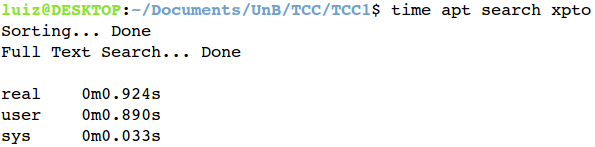
\includegraphics[width=0.8\textwidth]{figuras/xpto}
  \caption{Exemplo do uso do comando {\code time}}
  \label{fig:figuras_xpto}
\end{figure}


\subsection*{Mantendo uma cópia para a contribuição} % (fold)
\label{sub:mantendo_uma_copia_sua}

Normalmente não temos autorização pra alterar as informações de outra pessoa sem seu o consentimento. Da mesma forma  acontece com os repositórios {\code git}. Assim, um dos primeiros passos para começar a contribuir com uma ferramenta \textit{open-source} é fazer uma cópia dela em seu repositório. Essa cópia pode ser feita basicamente de duas formas, no intuito de preservar os autores das modificações anteriores:

\begin{description}
	\item [\textit{Fork}]: O termo é amplamente utilizado quando queremos fazer uma copia de um repositório para a nossa conta em uma mesma plataforma. Normalmente este passo é realizado via interface gráfica, ainda no navegador. Na \autoref{fig:github_fork} é possível observar o botão no canto superior direito que permite realizar um \textit{fork} do repositório desejado.

	\begin{figure}[h]
	  \centering
		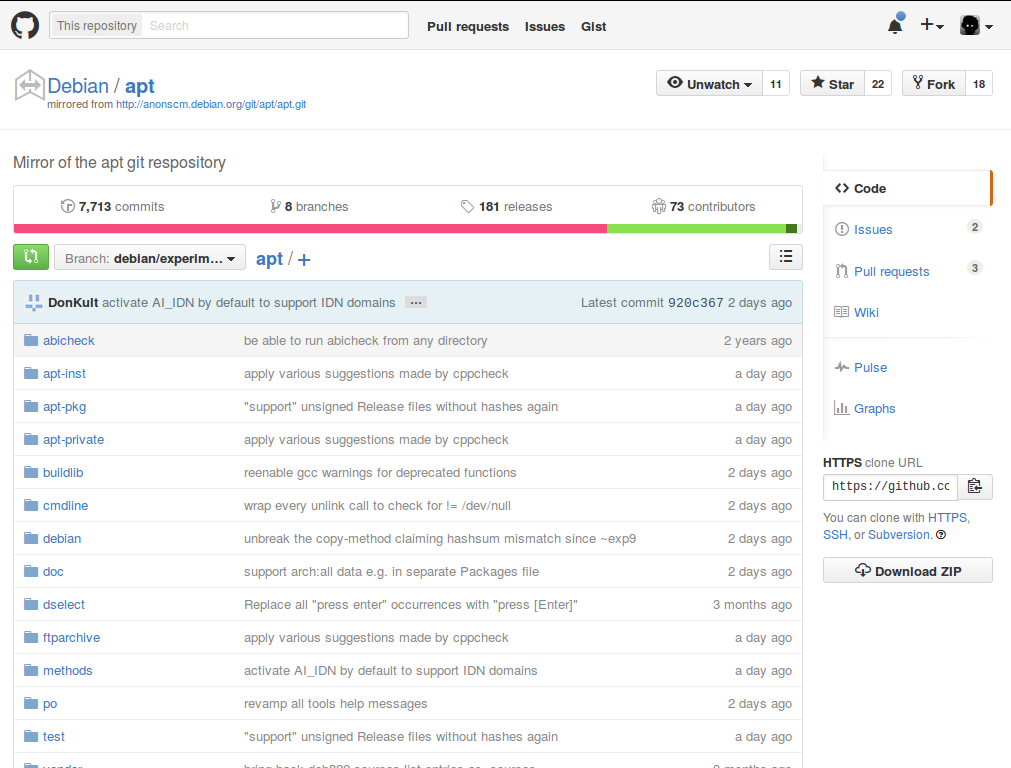
\includegraphics[width=0.90\textwidth]{figuras/fork}
	  \caption{Visão de um repositório do \textit{GitHub}, com destaque no botão que permite criar um \textit{fork} do projeto}
	  \label{fig:github_fork}
	\end{figure}

	\item [\textit{Adicionando \textit{remote}}]: Quando desejamos realizar uma cópia do repositório em uma plataforma distinta da original, a forma mais simples de proceder é clonando o repositório e incluindo nele um novo \textit{remote} para a nova plataforma. O \textit{remote} é o \textit{link} do repositório utilizado para a transmissão das alterações. Ele pode oferecer uma conexão {\code hhtps} ou {\code ssh}. Assim conseguimos trabalhar com a mesma árvore de \textit{commits} do repositório original, mantendo os créditos e alterações originais.
\end{description}
% subsection mantendo_uma_copia_sua (end)

\subsection*{Evoluindo o código} % (fold)
\label{sub:evoluindo_o_c_digo}

Nesto ponto de contribuição, o contribuinte desenvolve o código de acordo com o processo de produção escolhido. O código estará versionado em um repositório pessoal e o usuário possuirá todos os direitos administrativos deste repositório. Obviamente, caso a contribuição esteja sendo feita à uma aplicação grande e com muitos contribuidores, é importante se manter sincronizado com o código original, para evitar que o retorno da contribuição não seja tão trabalhoso para o revisor, além de evitar situações de conflito.
% subsection evoluindo_o_c_digo (end)

\subsection*{Retornando sua contribuição} % (fold)
\label{sub:retornando_sua_contribui_o}

Quando se decidido que a contribuição atinge um ponto aceitável para ser incorporada ao código original, é o momento de se realizar o \textit{pull-request}\footnote{Ou \textit{merge-request} dependendo da plataforma de desenvolvimento.}. Uma contribuição é interessante quando possui as seguintes características:


\begin{itemize}
	\item É uma significativa e relevante evolução de código mantendo os padrões de guia de estilo definido pelo desenvolvedor original/linguagem;
	\item Adiciona ou atende os testes para a evolução de código proposto;
	\item Traz a documentação da \textit{feature} implementada ou atualiza a documentação para contemplar as modificações sugeridas.
\end{itemize}
% subsection retornando_sua_contribui_o (end)

Submetida a contribuição, é dever do mantenedor do repositório original revisar o código e decidir se deve ou não aceitá-la.


\subsection*{Testando} % (fold)
\label{sub:testando}

É desejável, no desenvolvimento de software, existir um conjunto de testes unitários a cada evolução de código, a fim de validar as funcionalidades existentes ou adicionadas. No projeto abordado neste trabalho, em especial, há testes utilizado o \href{https://github.com/google/googletest}{Google C++ Testing Framework}\footnote{Disponível em \url{https://github.com/google/googletest}.} (Google Test), um \textit{framework} desenvolvido pela Google para testes. Ele tem suporte para um conjunto de assertivas pré-definidas e definidas pelo usuário, tornando-se uma das melhores ferramentas para a escrita de conjuntos de testes para C/C++ hoje disponíveis.

Outra categoria de testes se refere aos testes de integração. Neste trabalho em especial estará sendo utilizado um \textit{shell script} que oferece diversas funcionalidades para a criação dos testes de integração. Os testes de integração são utilizados no {\code APT} como testes caixa preta, a fim de verificar as funcionalidades em cenários de testes.

Os testes de integração tem maior prioridade que os unitários no APT, e podemos observar isso pela quantidade de testes em cada um deles. Nos testes unitários temos 20 casos de teste, totalizando 78 testes. Já nos testes de integração temos um conjunto de 199 cenários de testes, em um total de 24.976 testes\footnote{Dados relativos a \textit{build} \#219 do \href{https://travis-ci.org/Debian/apt/builds/}{Travis-CI}, em \url{https://travis-ci.org/Debian/apt/builds/}.}.


\begin{lstlisting}[language=C++,label=gtestexample,caption={Teste de validação de armazenamento de parâmetros}]
TEST(CommandLineTest,SaveInConfig)
{
   EXPECT_CMD("apt-get install -sf",
	 "apt-get", "install", "-sf");
   EXPECT_CMD("apt-cache -s apt -so Debug::test=Test",
	 "apt-cache", "-s", "apt", "-so", "Debug::test=Test");
   EXPECT_CMD("apt-cache -s apt -so Debug::test=\"Das ist ein Test\"",
	 "apt-cache", "-s", "apt", "-so", "Debug::test=Das ist ein Test");
   EXPECT_CMD("apt-cache -s apt --hallo test=1.0",
	 "apt-cache", "-s", "apt", "--hallo", "test=1.0");
}
\end{lstlisting}

Um exemplo de teste unitário realizado é a validação do armazenamento dos parâmetros nas chamadas, como pode ser observado no \autoref{gtestexample}. Já testes de integração possuem um comparativo entre uma chamada e sua saída, como pode ser observado no \autoref{integrationtesteexample}.

\begin{lstlisting}[language=Bash,label=integrationtesteexample,caption={Teste de verificação de saída para busca}]
# without op progress
testsuccessequal "foo/unstable 1.0 all
  $DESCR
" apt search -qq xxyyzz
\end{lstlisting}

% subsection testando (end)
% section contribuindo_com_plataformas_abertas (end)


\subsection{Coleta de Dados} % (fold)
\label{cha:coleta_de_dados}

\subsection*{Tempo} % (fold)
\label{sec:tempo}

A coleta de tempo de performance de um software é uma tarefa árdua. A estimativa de tempo depende das otimizações que o compilador pode vir a fazer para a arquitetura, memória disponível, aplicativos rodando em \textit{background}, temperatura do hardware, etc. No intuito de simplificar o processo de estimativa de tempo, foi utilizado a mediana de uma série de execuções da aplicação. Assim, o \autoref{scriptods} foi uma solução desenvolvida para deixar a maquina dedicada para a aquisição de dados com base no nome das \textit{branchs} e na lista de pacotes selecionados.

Para o funcionamento do \textit{script}, as variáveis {\code MAX} e {\code \_MAX\_THREADS} devem ser definidas com a quantidade de dados que se deseja coletar e a quantidade máxima de \textit{threads} que devem ser criadas para a chamada do processo, respectivamente. Usar uma quantidade superior à quantidade de \textit{cores}  da máquina pode produzir valores com baixa confiabilidade, visto a concorrência gerada pelas próprias \textit{threads}. Como parâmetros, foram escolhidos $150$ dados com $7$ \textit{threads}, deixando ao menos $1$ \textit{core} livre. Para maior dinamismo na coleta dos dados, o \textit{script} é responsável por realizar a troca das \textit{branchs} onde estão localizadas as possíveis soluções e a compilação e registro dos dados em uma planilha do \textit{LibreOffice Calc}. Assim, os algoritmos nunca são executados paralelamente, porém os dados serão coletado sob a demanda da $CPU$ na qual o \textit{script} é executado.

Para coletar o tempo de execução do algoritmo, o \autoref{libtime} foi desenvolvido a fim de ser usado como cronômetro. O algoritmo desenvolvido com o auxilio da biblioteca {\code Chrono}\footnote{Disponibilizada no {\code C++11} sob o \textit{namespace} {\code std::crono}.} permite a captura do intervalo de tempo com até $9$ casas decimais (nanosegundos), todavia foi utilizado a precisão de microssegundos ($10^ 6$) apenas, visto que o intervalo de nanosegundos não implicou em diferença significativa dos valores. Os métodos {\code begin()} e {\code end()} da classe são utilizados para pontuar os intervalos onde o tempo deve ser registrado. O resultado da medição pode ser obtido com o retorno do método {\code end()} ou com a chamada do {\code currenttime()}, dedicado apenas ao retorno deste valor.

\subsection*{Memória}

Para a coleta de memória, foi utilizado o {\code Valgrind}, com o auxílio da ferramenta {\code Massif}. Devido a criação da \textit{hash} ser feita de forma  algébrica e o método de \textit{KMP} utilizar um autômato finito determinístico, a repetição prévia das buscas com apenas $10$ amostras confirmavam a suspeita de não haver a variação do gasto de memória.

Para a execução da aplicação com o suporte ao {\code Valgrind} para análise do uso de memória, foi utilizado o comando:

\begin{lstlisting}[language=Bash,label=valgrind_call, numbers=none]
   $ valgrind --tool=massif  ./apt search pacote [--regex]
\end{lstlisting}
% section tempo (end)
% chapter coleta_de_dados (end)


\subsection{Ferramentas}

Para a realização desta contribuição as seguintes tecnologias estiveram envolvidas:

\begin{description}
	\item[Sublime-Text] Editor de texto.
	\item[Vim] Editor de texto.
	\item[Git] Sistema de controle de versão.
	\item[Make] Ferramenta de execução de comandos {\code bash}.
	\item[GCC] Compilador de C/C++.
	\item[Mint] Distribuição Linux baseada em Debian.
\end{description}

Os serviços das seguintes organizações também foram utilizados na produção deste trabalho:

\begin{description}
	\item[Github] Oferecem serviço de hospedagem de repositórios.
	\item[Travis CI] Oferecem serviço de Integração Continua.
\end{description}

Para desenvolvimento, foi utilizado uma maquina com as seguintes configurações:

\begin{description}
	\item[OS:] Mint 17.1 Rebecca
	\item[Kernel:] x86\_64 Linux 3.13.0-37-generic
	\item[CPU:] Intel Core i7 CPU 870 @ 2.934GHz
	\item[GPU:] GeForce GTX 465
	\item[RAM:] 12Gb
\end{description}

Durante o desenvolvimento, as seguintes versões das ferramentas foram utilizadas:

\begin{description}
	\item[]\textbf{GCC} - 4.8.4
	\item[]\textbf{GIT} - 1.9.1
	\item[]\textbf{Make} - 3.81
	\item[]\textbf{APT}
	\begin{itemize}
		\item\textbf{local:} 1.0.1ubuntu2
		\item\textbf{repositório:} 1.1~exp14
	\end{itemize}
\end{description}
 